\section{CLI app}\label{sec:cli-app-contents}

\subsection{CLI app improvements}\label{subsec:cli-app-improvements}
Our CLI app is based on~\nameref{subsec:git-time-metric}, an already working open source time tracking app.
Although it already had all the basic features, some improvements and fixes were required.

Firstly \textit{--cwd=\{some/path\}} option was added to allow easier integration of plugins.
Option to pass current directory as option is required, as IDEs not launched from terminal sometimes have their working
directory elsewhere and setting custom working directory every time we call CLI app is more complicated than passing an argument.

To clean up user home directories, global config files were moved from \textit{~/.git-time-metrics/} to \textit{~/.config/gtm/}.
For windows a new installer was built to make installing easier.
Also, it was chosen to switch from statically compiling SSH2 Libraries into our application to dynamic linking.
For Debian Linux, a build script for debian packages was set up to also provide debian packages with every release.

The application was updated to automatically add a fetch refspecs to fetch data from remotes on git fetch.
Also, a pre-push git hook was added to automatically push data to origin.
With these two hooks, the time data is automatically fetched pushed whenever git push is made requiring user no extra effort.

To still allow users to only track time locally, a \textit{--local} option was added to \textit{init} command.
Also \textit{--auto-log=[jira|gitlab]} option was added to support automatic time logging to commit messages.
Currently, this time can only be collected in Jira, but there is also and \href{https://gitlab.com/gitlab-org/gitlab/-/issues/16543}{issue}
open for Gitlab to implement this.\cite{gitlab-time-issue}

To view data based branch the checked out branch name when the commit was made is also now stored to data.
This couldn't be avoided because the branch is simply a pointer to commit and due to git being distributed control system,
it isn't guaranteed.

For students, it is important to view time spent on specific tasks.
In most subjects the tasks are placed in separate subdirectories for better files management.
To allow users to view time spent on specific tasks, a \textit{--subdir="sub/dir/name"} option was added to filter out
data based on directories.

Although the Git supports automatic merging/rewriting of the notes, it was inconsistent in some cases, especially when the user
wants to also rewrite manually added notes.
To keep time data after Git rebases, a new command \textit{rewrite} was introduced.
This command is ran by git post-rewrite hook, and it rewrites notes so that they still point to correct commit.

\subsection{Initializing tracking}\label{subsec:init-tracking}
Main flow for initializing tracking for repository is described in Figure~\ref{fig:init-tracking}.
\begin{figure}[h]
    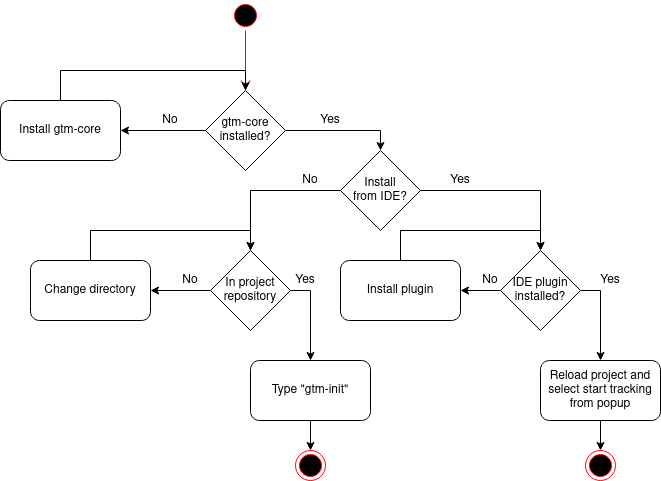
\includegraphics[width=\textwidth]{figures/init_tracking}
    \caption{Initialize tracking}
    \label{fig:init-tracking}
\end{figure}

First requirement is that you need to have gtm-core installed and added to \textit{PATH} in order to initialize tracking.
If the user has gtm-core installed he can initialize tracking from command line.
To do that, it is required to change your current directory to be somewhere within git root directory.
Time tracking is then initialize with \textit{gtm init} command.
The command support following arguments:

\begin{table}[h]
    \centering
    \begin{tabular}{ | p{3cm} | p{10cm} |}
        \hline
        Argument & Description\\
        \hline
        --terminal & Enable time tracking for terminal. (Requires terminal plugin)\\
        \hline
        --auto-log & Either \textit{gitlab} or \textit{jira} to automatically log time
        into commit messages with given format.\\
        \hline
        --local & If set, no git fetch nor push hooks are added.
        Time data is only stored locally.\\
        \hline
        --tags & Optionally add tags to project for better local organization.\\
        \hline
        --clear-tags & If project already has some tags running it with given flag removes previously added flags.\\
        \hline
        --cwd & Useful for specifying working directory for scripts.\\
        \hline
    \end{tabular}
    \caption{Gtm-front folder structure.}
    \label{tab:gtm-init}
\end{table}
It is safe to run \textit{gtm init} multiple times with any of the arguments.

The user can also initialize time tracking from within IDE if he has gtm plugin installed.
Currently, only Jetbrains IDE plugin support starting tracking.
To initialize time tracking from Jetbrains IDE the user needs to open/reload project he wishes to add time tracking to.
Upon doing that he is prompted to choose whether to start tracking or not.
To initialize tracking, start tracking has to be chosen.
This initializes tracking for currently open repository with default settings (equal to no argument for CLI).
If the user chooses not to initialize tracking, his choice is persisted in local project file within \textit{.idea} directory.
To later add tracking to repository, he needs to do it from command line or by deleting project settings file.


\section{IDE Plugins}\label{sec:plugins}

IDE plugins are used to capture editor specific events and then execute appropriate commands on gtm-core.
Basically gtm-core and IDE plugin combo works like a language server and code formatting plugin combo.
This eliminates need to write duplicate code when writing plugins for multiple IDEs.
Currently, we have full support for Jetbrains and some support for Vim.
There are also many more plugins that have been previously written for original Git-Time-Metric, and most of them also work with our app.

\subsection{Jetbrains}\label{subsec:jetbrains-plugin}
Jetbrains also had plugin for original Git-Time-Metric, but the IDE has gone through lots of changes since the last update to plugin.
As of 2021 this causes Jetbrains IDEs to crash.
We decided to fully rewrite the plugin as it heavily used now deprecated Jetbrains components.

The plugin catches following events and forwards the data to gtm-core:
\begin{enumerate}
    \item Opening file in editor.
    \item Mouse pressed inside editor (on file).
    \item Process run (Mostly build, test, debug or run, but can be any other process you run via IDE)
    \item File saved.
    \item Visible area changed (Window resized / split).
\end{enumerate}

In response, plugin gets time since last commit (uncommitted time), which it show on the bottom status bar.

In addition to silently listening for events and updating time the plugin communicates with user via popup dialog and notification.
The popup dialog is used to prompt user whether he wants to start tracking time for project as described in~\nameref{subsec:init-tracking}
Notifications are used to report errors and more important actions results (such as whether adding tracking was successful).

\subsection{Vim}\label{subsec:vim-plugin}
Already existing \href{https://github.com/git-time-metric/gtm-vim-plugin}{plugin} for vim was forked as it had all the required features.
Version numbers and update links were changed to comply with our version.
As the Vim script file to give the support for tracking time and also displaying it on status line is under 80 lines long
it perfectly describes, why it was necessary to have gtm-core as a separate program instead of writing the business logic inside plugin.


\subsection{Adding tracking to repositories}\label{subsec:adding-tracking}
We have added three levels to view time data:
\begin{enumerate}
    \item Add tracking (locally), view data via gtm CLI app.
    \item Add tracking (locally), log data to commit messages.
    \item Add tracking, sync data to gtm Web App.
\end{enumerate}

All smaller level can be included while using higher level option.
Viewing data via CLI app is always possible, as it is the same app that is responsible for recording data.
This can be done both only locally or with pushing and pulling notes from remotes.
You can also add logging time spent to commit messages in both of the scenarios as it simply works on top of the already
existing system and only modifies commit message.
To use auto logging option you simply need to add \textit{--auto-log=[gitlab|jira]} option when initiating tracking for a repository.

To view data from web interface, some more steps are required.
User flow for making repository visible on gtm web application is shown on Figure~\ref{fig:add-tracking-user-flow}.

\begin{figure}[h]
    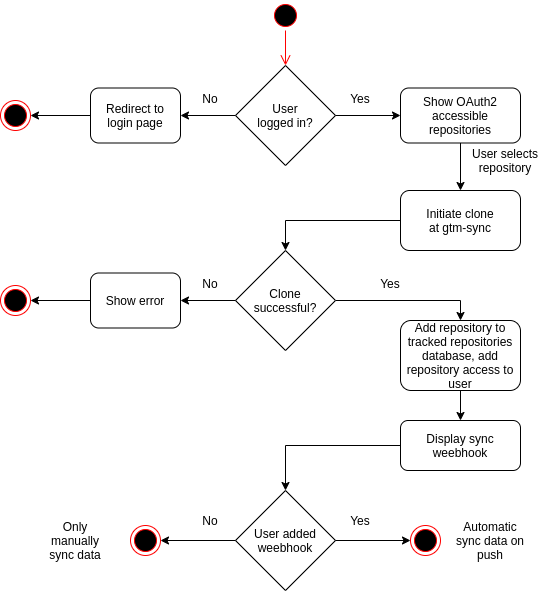
\includegraphics[width=\textwidth]{figures/add_repo_user_flow}
    \caption{Add tracking user flow}
    \label{fig:add-tracking-user-flow}
\end{figure}

Firstly, to have our sync client access the data, you cannot have time data only stored locally.
Then to add a repository, you need to have linked appropriate git server provider account via OAuth so that we can
verify that you have the access to repository.
After that you need to search for the repository from web interface and click add tracking button.
With that the tracking is technically added, but to also automatically sync time data on every push to remote,
you also need to add webhook.

To make sure that the repository can be accessed by the user the request to appropriate provider is made again
when user has pressed \textit{"Start tracking"} button.
This check is required as the user could easily guess other peoples private repository clone urls and then post
it to our backend with his own JWT.
This extra check also means you cannot add tracking to self-hosted git servers that do not provide OAuth2.
However, we could not find any better way to identify that the given user has access to some git repository and
therefore it was decided to not support any custom setups.

\section{Backend}\label{sec:backend-content}

Sync client which has api key registered has access to the endpoints in Table~\ref{tab:gtm-api-endpoints-for-sync}.
\begin{table}[h]
    \centering
    \begin{tabular}{ | p{4cm} | p{4cm} | p{4cm} |}
        \hline
        Endpoint & Parameters & Description\\
        \hline
        POST /repositories & - & Sync client can send new repo timeline data \\
        \hline
        PUT /repositories & - & Sync client can send existing repo updated timeline data\\
        \hline
        GET /commits/hash & provider: string, user: string, repo: string & Returns last commit hash, timestamp and tracked commit hashes\\
        \hline
    \end{tabular}
    \caption{Gtm-api endpoints for sync client.}
    \label{tab:gtm-api-endpoints-for-sync}
\end{table}

An authorized user has access to the endpoints in Table~\ref{tab:gtm-api-endpoints-secured}.
\begin{table}[h]
    \centering
    \begin{tabular}{ | p{4cm} | p{4cm} | p{4cm} |}
        \hline
        Endpoint & Parameters & Description\\
        \hline
        GET /groups & - & Returns all the groups logged-in user has access to. \\
        \hline
        GET /\{group\_name\}/activity & start: int, end: int, interval: string, timezone: string & Returns activity for group. \\
        \hline
        GET /\{group\_name\}/subdirs-timeline & start: int, end: int, interval: string, timezone: string, depth: int & Returns sub-directory timeline for group. \\
        \hline
        GET /\{group\_name\}/timeline & start: int, end: int, interval: string, timezone: string & Returns timeline for group. \\
        \hline  % TODO: Group stats endpoint
    \end{tabular}
    \caption{Gtm-api secured public endpoints}
    \label{tab:gtm-api-endpoints-secured}
\end{table}

Unauthorized user has access to the endpoints in Table~\ref{tab:gtm-api-endpoints-public}.
\begin{table}[h]
    \centering
    \begin{tabular}{ | p{4cm} | p{4cm} | p{4cm} |}
        \hline
        Endpoint & Parameters & Description\\
        \hline
        POST /auth/login & - & For login \\
        \hline
        POST /auth/register & - & For registering new account \\
        \hline
    \end{tabular}
    \caption{Gtm-api not secured public endpoints.}
    \label{tab:gtm-api-endpoints-public}
\end{table}

All the endpoints can be found \href{https://cs.ttu.ee/services/gtm/api/swagger/index.html}{here}.

\subsection{Security}\label{subsec:scurity}
Our application holds data, that shall not be visible to all client and therefore some kind of authentication and authorization methods are required.
For the data stored in Git notes we decided no extra security is required, as the time data isn't more sensitive than the actual code.
The security of source code stored in git repository is handled by a client himself and Git providers.
If they wish to have some more protection for git notes, they can configure it themselves.
We only provide the option to have notes only stored locally (not pushed to origin).

For the web application we need to implement our own security measures.
For most basic usage we have simple username and password authentication.
Accounts that only have password authentication are not authorized to access any groups nor repositories unless Admin user
explicitly gives them access to any.

To automatically get access to repositories you are contributor of you need to authenticate yourself via OAuth2 standard.
This way we can verify, that the user signing in to our application is the same user that has access to some git repository.

\subsubsection{OAuth2}\label{subsubsec:oauth2}
For OAuth2 authorization rocket{\_}oauth2 library is used, that follows RFC-6749 standard~\cite{rocket-oauth2, oauth2}.
We support authentication via \href{https://github.com/}{Github.com}, \href{https://about.gitlab.com/}{Gitlab.com},
\href{https://bitbucket.org/}{Bitbucket.org}, \href{https://azure.microsoft.com/}{Azure} (Microsoft account) and
TalTech \href{https://gitlab.cs.ttu.ee/}{gitlab server}.
First three were chosen as they are the most common git server providers as of 2021.
Authentication via Microsoft was added as TalTech (and also numerous other universities / companies) use it and therefore
all students have already registered account there.
Also, it provides access to user emails, that can be later used to filter out user commits.
TalTech gitlab server was added, as the application is currently developed for TalTech and therefore it was a requirement
that everything shall also work on TalTech gitlab server.

From all OAuth2 providers at least user read access is required to get access to user emails.
For OAuth2 providers, that are also a Git server providers also permissions to read user repositories data is required.
User repositories data is used to give user automatically access to his own repositories and also display repositories
not currently tracked by gtm.
It also allows more easily adding automatic data collection to user repositories, as user can browse through
repositories from different git server providers.

\subsection{Groups system}\label{subsec:group-system}
One of the requirements for our app was that it should be possible to group repositories together.
The grouping is needed to view statistics for multiple repositories at once and also compare groups of repositories.
The grouping system should be also capable of controlling user access rights to different repositories.

Requirements for grouping system
\begin{itemize}
    \item It shall be possible to group both repositories and groups already consisting of repositories.
    \item Single repository may be possible of multiple groups.
    \item Group access can be limited to only viewing summary (group total).
    \item Granting user an access group subgroups and then removing it shall have no side effects. (Accesses to subgroups shall not be persisted)
\end{itemize}

As the groups may consist of both groups and repositories we decided to automatically create group for every repository.
This means now groups can only consist of zero or more other groups.
If we need te get the repository we can fetch all the group ids that are accessible and then query from repositories database by
comparing repositories group id against previously fetched ids.
To fetch group with all of its subgroups a recursive Structured Query Language (SQL) query was needed as the groups'
hierarchy formulates a tree like structure.
Our database provider PostgreSQL supports recursive queries so there were no technical problems with implementing it on SQL database.
A simplified version of our group system database tables can be seen of Figure~\ref{fig:group-system}

\begin{figure}[h]
    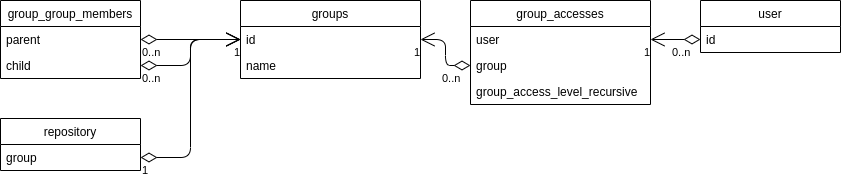
\includegraphics[width=\textwidth]{figures/group_system}
    \caption{Application groups system}
    \label{fig:group-system}
\end{figure}

This tree like groups' hierarchy allows us to easily give and take user access to any group.
If we want to change access from only parent group to also all subgroups access, we can simply toggle access{\_}level{\_}recursive
variable.
If we remove one particular group access, all other accesses remain in place, meaning that you some group was accessible
also via some other group access, you still have the access.

\subsection{Roles}\label{subsec:roles}
Our application has three different roles to control user permissions.
Single user can belong to multiple roles and roles and also new roles can be dynamically added to database as they are
kept in separate table.
Currently, there are three roles in total: \textit{USER}, \textit{LECTURER} and \textit{ADMIN}.
Role \textit{USER} is added to every created user, and it has no extra permissions.

People with \textit{USER} role can:
\begin{enumerate}
    \item View data from git repositories, they have access to.
    \item Add new repositories.
    \item Delete repositories they have access to.
\end{enumerate}

People with \textit{LECTURER} role can:
\begin{enumerate}
    \item View data from git repositories, they have access to.
    \item Add new repositories.
    \item Delete repositories they have access to.
    \item Give access to others.
\end{enumerate}

People with \textit{ADMIN} role can:
\begin{enumerate}
    \item Assign new roles to other users.
    \item View data from all the repositories and groups.
    \item Give other users group accesses.
\end{enumerate}

\section{Frontend}\label{sec:frontend-content}
Frontend is one-page web application.
Users can log in and see their data according to their privileges.
This application has two main parts - profile and data visualization.
Under profile users can change password, link OAuth accounts and delete account and add repositories.
Data visualization is divided into 3 parts - dashboard, leaderboard and timeline comparison.
In those tabs users can see their/others data as graphs and tables.

\subsection{Authentication and authorization}\label{subsec:authentication-and-authorization}
Authentication and authorization is implemented using bearer token system.
User gets JSON Web Token from api and stores it to the localstorage and adds to every request header.
User has to log in from log in page.
On success client receives JSON Web Token from backend and client stores it in localstorage.
Then user is automatically redirected to main page.
Users can log in with OAuth or username/password.
In case of OAuth user is redirected to according OAuth platform for authentication.
When successful, user is redirected to frontend with JSON Web Token (JWT).
JSON web token is saved on localstorage and user is redirected to main page where he/she can access their data.
Login and register user flows are described on Figure
\ref{fig:login-signup-diagram}.

\begin{figure}[h]
    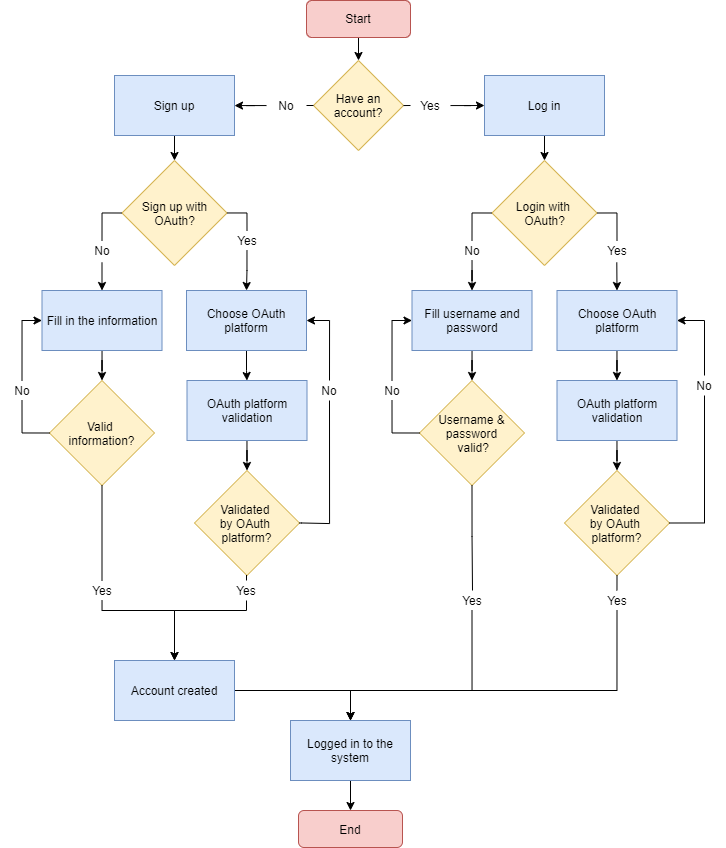
\includegraphics[width=\textwidth]{figures/login_signup_diagram}
    \caption{Log in and sign up flows}
    \label{fig:login-signup-diagram}
\end{figure}

\subsection{Profile}\label{subsec:profile}
\subsubsection{OAuth linking}\label{subsubsec:oauth-linking}
It is also possible to link multiple OAuth platforms to one account.
In that case user has to log in and head to the profile page where he/she can find link accounts tab.
If OAuth platform is already linked then backend unlinks it from this account, otherwise user is redirected to OAuth platform for authentication.
On success user will be redirected to frontend and user can access new repositories that this OAuth platform account has.
OAuth linking flow is described on Figure
\ref{fig:account-linking}.

\begin{figure}[H]
    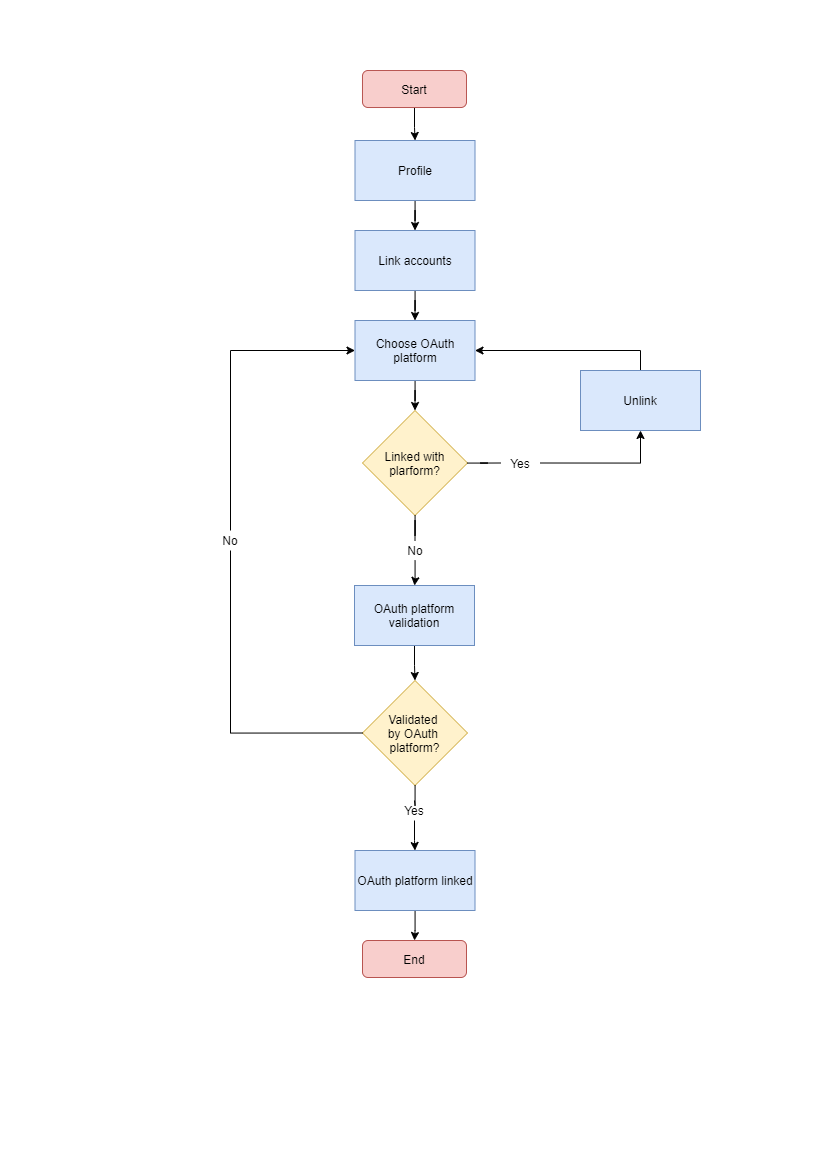
\includegraphics[width=\textwidth]{figures/account_linking}
    \caption{OAuth linking with user}
    \label{fig:account-linking}
\end{figure}

\subsubsection{Change password}\label{subsubsec:change-password}
Users can also change password.
In profile view under change password tab user has to fill all the fields correctly and password will be changed.
If user does not have a password (OAuth registration), only new password fields have to be filled.
Once you have already added a password, it's not possible to remove it to avoid possibility to have inaccessible accounts.

\subsubsection{Repositories}\label{subsubsec:repositories}
Under repositories tab user can see all their repositories.
User can start tracking new repository by clicking start tracking and then adding webhook to according OAuth platform.
If start tracking is clicked and everything is successful, a blue info box with instructions for webhook will pop up.
In case user wants to start tracking again then the repository can be found at the end of the list with button initialize again.
Tracking can also be stopped by clicking on the red button with trash can.
% TODO lisasse screenshot

\subsubsection{Delete account}\label{subsubsec:delete-account}
Account deletion is under delete account tab.
To keep away accidental account deletion user has to write their name to the input box and then can submit.
If account is deleted, user is redirected to the login page.
% TODO: Mis siis kui viimase OAuthi unlinkid? ka delete? tegelt vist oleks warning vms parem aga idk

\subsection{Data visualization}\label{subsec:data-visualization}
Data visualization is divided into three pages - dashboard, leaderboard and comparison.
From sidebar user can navigate to necessary page and on top of the page user has selection of properties according to the graphs.

\subsubsection{Dashboard}\label{subsubsec:dashboard}
Dashboard is the main landing page if user is logged in.
Dashboard contains three graphs and inputs.
From inputs user can change group, time period and interval.
User can choose between all the groups he/she has access to.
Time period has start and end which cannot be apart more than a year for performance reasons.
Intervals are days, weeks and months.

First graph is a combination of line and bar charts which describes time spent in time and also shows how many users were active at the interval.
X-axis shows the period of time and Y-axis on shows the time spent during the period.
Y-axis also shows active users count during the period.
Line shows time spent and bar shows users count.

Second graph is line chart which describes activity hours during the chosen period.
According to the interval it shows daily activity, weekly activity or monthly activity.
X-axis shows interval and Y-axis shows average time spent during this time.
If interval is day then X-axis describes each hour, in case of week, X-axis describes each week day, etc.
Y-axis also shows lines added and removed from code.
This graph brings out the timeframe when users are actively programming.

Third graph is bar chart which describes time spent in folders or files.
X-axis shows the period of time and Y-axis shows the time spent during the period.
Bars are stacked on each other and each bar describes one folder or file.
This graph brings out on which tasks people spend most of their time on and is very useful for lecturers who want to see which homeoworks take more time.

\subsubsection{Leaderboard}\label{subsubsec:leaderboard}
Leaderboard contains four inputs and two tables where users and files/folders can be easily compared.
Inputs contain group selection, date selection and depth selection.
Depth determines how deep will the search go for files and folders.

First table shows info about users in chosen group.
Data is divided into 7 columns - total time, commits, lines added, lines removed, lines per hour, commits per hour and lines per commit.
By clicking on the column header the sequence will change accordingly.

Second table shows info about file system.
Data is divided into 8 columns - total time, commits, lines added, lines removed, lines per hour, commits per hour, lines per commit and users.
Sequence can also be changed by clicking on the column header.
This table can be useful for comparing different tasks in university as they are usually placed in separate folders.

At the end of the page there is export data button which downloads csv file with data.

\subsubsection{Comparison}\label{subsubsec:comparison}
Comparison page has four inputs and one graph.
Inputs again are group selection, date selection and interval selection.
Multiple groups can be selected to compare them.
Graph draws out lines charts depending on amount of groups selected.
X-axis shows the period of time and Y-axis shows time spent.
Each line has different color as it represents different group and makes the graph more understandable.
